\documentclass{standalone}
\usepackage{tikz}
\usepackage{ctex,siunitx,ninecolors}
\setCJKmainfont{Noto Serif CJK SC}
\usepackage{tkz-euclide}
\usepackage{amsmath}
\usetikzlibrary{patterns, calc}
\usetikzlibrary {decorations.pathmorphing, decorations.pathreplacing, decorations.shapes,}
\begin{document}
\small
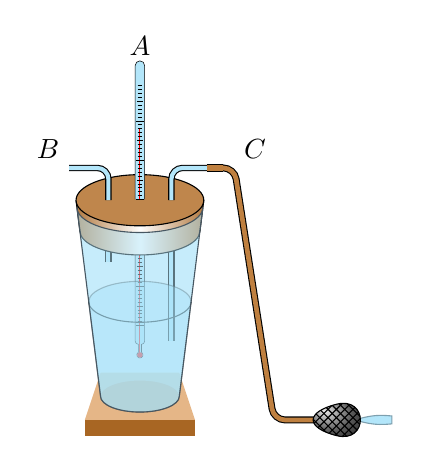
\begin{tikzpicture}[>=latex,scale=1.0]
  % \useasboundingbox(-1.4,-1.4)rectangle(1.4,1.4);
  \fill[brown8](-0.7,0)--(0.7,0)--(0.5,0.6)--(-0.5,0.6);
  \fill[brown5](-0.7,0)rectangle(0.7,-0.2);
  \fill[cyan!40!gray,opacity=0.3](0,0.3)ellipse(0.5 and 0.2);
  \fill[cyan!30,opacity=0.5](-0.8,2.7)arc(180:0:0.8 and 0.32)--(0.5,0.3)arc(0:180:0.5 and 0.2);
  \draw[double=cyan!30!white,double distance=1.5pt](-0.4,2)--(-0.4,2.4);
  \draw[double=cyan!30!white,double distance=1.5pt](0.4,1.0)--(0.4,2.4);

  \draw[fill=cyan!30!white,very thin](-0.06,2.4)--(-0.06,1.0)arc(-180:-90:0.04)--++(0,-0.1)arc(120:420:0.04)--++(0,0.1)arc(-90:-0:0.04)--(0.06,2.4);
  \fill[red](0,0.825)circle(0.035);
  \node at (0,4.5)[above]{$A$};
  \draw[red](0,0.825)--(0,2.4);
  \foreach \y in {1,1.5,2}
  {
    \draw[ultra thin](-0.05,\y+0.2)--++(0.1,0);
    \draw[ultra thin](-0.04,\y+0.45)--++(0.08,0);
    \foreach \z in {1,2,3,4,6,7,8,9}
    {
      \draw[ultra thin](-0.03,\y+0.2+0.05*\z)--++(0.06,0);
    }
  }
  \draw(-0.65,1.5)arc(-180:0:0.65 and 0.26);
  \fill[cyan!40,opacity=0.4,draw=black](-0.65,1.5)--(-0.5,0.3)arc(-180:0:0.5 and 0.2)--(0.65,1.5)arc(0:180:0.65 and 0.26);
  \draw[left color=brown!90!darkgray,right color=brown!90!darkgray,middle color=white](-0.8112,2.79)--(-0.7625,2.4)arc(-180:0:0.7625 and 0.305)--(0.8112,2.79);
  \draw[fill=brown!90!lightgray](0,2.79)ellipse(0.8112 and 0.3248);
  \draw[cyan!30!black,fill=cyan!30,fill opacity=0.5](-0.8,2.7)arc(-180:0:0.8 and 0.32)--(0.5,0.3)arc(0:-180:0.5 and 0.2)--cycle;
  \draw[fill=cyan!30!white,very thin](-0.06,2.8)--(-0.06,4.5)arc(180:0:0.06)--(0.06,2.8);
  \draw[red](0,2.8)--(0,3.7);
  \foreach \y in {2.6,3.1,3.6}
  {
    \draw[ultra thin](-0.05,\y+0.2)--++(0.1,0);
    \draw[ultra thin](-0.04,\y+0.45)--++(0.08,0);
    \foreach \z in {1,2,3,4,6,7,8,9}
    {
      \draw[ultra thin](-0.03,\y+0.2+0.05*\z)--++(0.06,0);
    }
  }

  \draw[double=cyan!30!white,double distance=1.5pt,rounded corners](-0.4,2.79)--(-0.4,3.2)--++(-0.5,0,0)node[above left]{$B$};
  \draw[double=cyan!30!white,double distance=1.5pt,rounded corners](0.4,2.79)--(0.4,3.2)--++(0.5,0);
  \draw[double=brown,double distance=1.7pt,rounded corners](0.9,3.2)--(1.2,3.2)node[above right]{$C$}--++(0.5,-3.2)--++(0.6,0);
  \draw[double=brown,double distance=2.2pt,rounded corners](0.85,3.2)--(1.05,3.2);
  \fill[cyan!30!white,draw=cyan!30!gray](2.8,0.02)to[bend left=10](3.2,0.05)--(3.2,-0.05)to[bend left=10](2.8,-0.02);
  \draw[ball color=gray](2.5,0.2)..controls(2.1,0.1)and(2.1,-0.1)..(2.5,-0.2)..controls(2.9,-0.3)and(2.9,0.3)..cycle;
  \fill[pattern=crosshatch](2.5,0.2)..controls(2.1,0.1)and(2.1,-0.1)..(2.5,-0.2)..controls(2.9,-0.3)and(2.9,0.3)..cycle;
\end{tikzpicture}
\end{document}